\documentclass[12pt]{article}
\usepackage{graphicx}
\usepackage{float}
  
%
% Title[Enter title of the experiment here]
\title{EE230: Experiment No.8\\
Logarithmic Amplifier}

% Author[Enter details of author here]
\author{Aksh Garg, 20D070008}

% begin the document.
\begin{document}

% make a title page.[this creates title page]
\maketitle
 

\section{Overview of the experiment} %[This segment creates Section as seen in document]

\subsection{Aim of the experiment}%[This segment creates sebsections under the same section]

The aim of this experiment is to understand Logarithmic Amplifier using op-amps (specifically TL084) about how it works and should be the circuit to implement this type of Amplifier. In this experiment, we have to find the linear region at which we can use the given circuit for our use, given the IV characteristics of the circuit. This circuit is simulated using NgSpice software, and these simulation results needs to be compared with the theoritical results.

\subsection{Methods}
First of all, the given IV characteristics are analyzed, we find the linear region to work upon the om-amp, and by using linear regression in python, we find the slope and the y-intercept (which is required for further calculations).\\
After that, circuit diagrams are made using XCircuit software of the required circuits. Now, as the circuits are formed, netlist codes are written for the circuit to completely describe the circuit and also describe what result ngspice should show to us. The readings are saved in a file and then, using this file, plots of the given parameters are made by matplotlib python script.\\
The lab work to be done was given in lab pdf, using that we got the circuit to be simulated.\\
After that, these plots were compared with the theoritical plot values and the changes are done to the circuit element values to refine the circuit.

\section{Design}%[To add multiple sections, keep appending blocks like this]

\begin{figure}[H]
\begin{center}
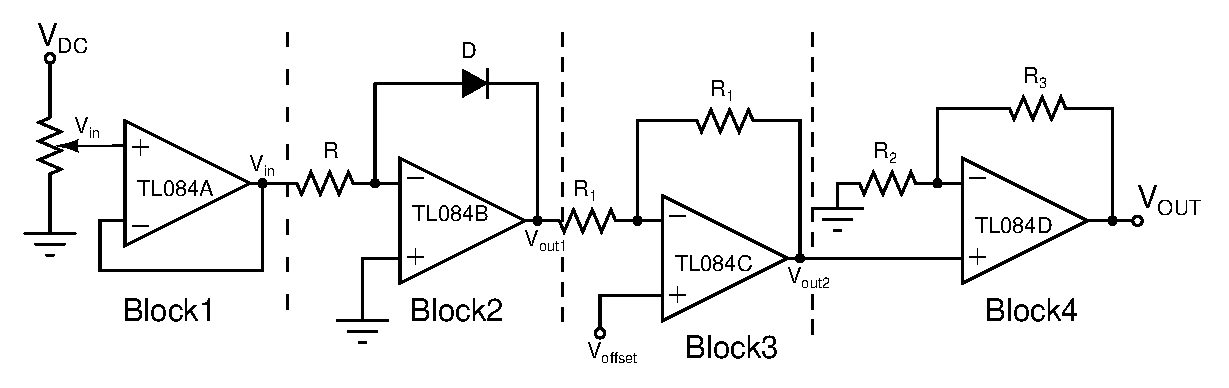
\includegraphics[scale = 0.8]{a.eps}
\end{center}
\end{figure}
The equation for the terminal characteristics of a pn junction diode in forward bias is
\begin{equation}
   I_D = I_S * e^{(V_D/nV_T)}
 \end{equation}
\begin{equation}
   V_D = nV_T  (ln(I_D) - ln(I_S)) 
 \end{equation}
\begin{equation}
  ln(I_D) = V_D/nV_T + ln(I_S)
 \end{equation}
\begin{equation}
  V_{out1} = -V_D
 \end{equation}
\begin{equation}
  V_{out1} = nV_T  (ln(I_SR) - ln(V_{in})) 
 \end{equation}
\begin{equation}
  V_{out1} = a_1 ln(V_{in}) + a_2 
 \end{equation}
\begin{equation}
 a_1 = -nV_T 
 \end{equation}
\begin{equation}
  a_2 = nV_T ln(I_SR) 
 \end{equation}

We can remove the offset by subtracting $a_2$ from $V_{out1}$. The result can then be multiplied by 1/$a_1$ using a suitable amplifier, to obtain at the output the true natural logarithm of $V_{in}$.\\
The third block is used for removing the offset from $V_{out1}$ , set $V_{offset}$ = $a_2$/2,  so the input to block 4 would be -$a_1$ ln($V_{in}$).\\
\begin{equation}
  V_{out} = -a_1(1 + R_3/R_2) ln(V_{in})  
 \end{equation}
Choosing 1 + $R_3$/$R_2$ = -1/$a_1$, we get
\begin{equation}
 V_{out} = ln(V_{in}) 
 \end{equation}
The role of block 1 is to avoid loading the source of $V_{in}$ by block 2.\\
If we assume that the maximum input voltage, $V_{in2}$ = 10V , then R = 10/$I_{D2}$.\\
\textbf{Values:-} \\
By observing the readings, we got linear region $I_D$ values from 1.266E-4 to 5.55E-4 Amperes.\\
So, 
\begin{equation}
 R =  10/I_{D2} = 18k\Omega 
 \end{equation}
By using linear regression in this region, we got slope = 20.5409, and y-intercept = -19.30584.\\
\begin{equation}
 Slope = 1/(nV_T)
 \end{equation}
\begin{equation}
 Y-intercept =  ln(I_S) 
 \end{equation}
\begin{equation}
 n  =1/(slope*V_T) = 1.87
 \end{equation}
\begin{equation}
 I_S  = e^{(y-intercept)} = 4.13nA
 \end{equation}
\begin{equation}
 a_1 = -(1.87)(26)/1000 = -0.04862
 \end{equation}
\begin{equation}
 a_2 = (1.87)(26) ln(4.13 * 18 /1000000) /1000 = -0.46
 \end{equation}

\begin{equation}
 V_{offset} = a_2/2 = (nV_T ln(I_SR))/2 = -0.23V
 \end{equation}
We set $R_1$ = 10k$\Omega $.
\begin{equation}
 R_3/R_2 = (-1/a_1) - 1 = 19.5
 \end{equation}
We set $R_2$ = 1k$\Omega $, and $R_3$ = 19.5k$\Omega $.\\
Now, we are done with all the calculations for finding the values of all the required values and parameters.



\section{Simulation results}%[One more section]
\subsection{Code snippet}

\begin{center}
\textbf{Logarithmic Amplifier}
\end{center}
\begin{center}
$V_{OUT}$ vs $V_{IN}$
\end{center}
.include TL084.txt\\
.include 1N4148.txt\\
x1 1 2 3 4 2 TL084\\
x2 0 5 3 4 6 TL084\\
x3 11 7 3 4 8 TL084\\
x4 8 9 3 4 10 TL084\\
r1 6 7 10k\\
rx 7 8 10k\\
r2 9 0 1.1k\\
r3 9 10 19.5k\\
r 2 5 18k\\
D 5 6 1N4148\\
vcc 3 0 15\\
vdd 4 0 -15\\
vin 1 0 dc 0 \\
vo 11 0 -0.219\\
.dc vin 0 10 0.1\\
.control\\
run\\
plot v(10)\\
print v(10)\\
.endc\\
.end\\

\begin{center}
$V_{OUT}$ vs ln($V_{IN}$)
\end{center}
This is done by using python.


\subsection{Simulation results}


\begin{figure}[H]
\begin{center}
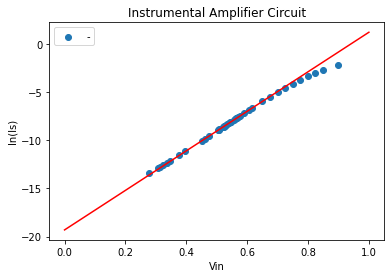
\includegraphics[scale = 0.8]{reg.png}
\caption{IV characteristics from the given data and also linear regression}
\end{center}
\end{figure}

\begin{figure}[H]
\begin{center}
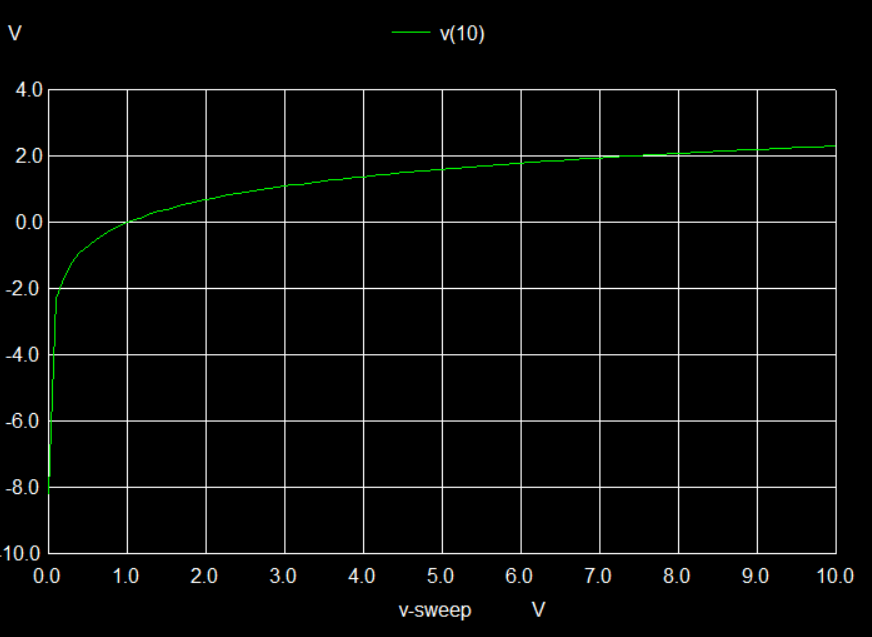
\includegraphics[scale = 0.5]{i.png}
\caption{$V_{out}$ vs $V_{in}$ (ideal)}
\end{center}
\end{figure}

\begin{figure}[H]
\begin{center}
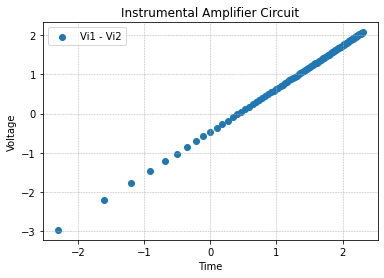
\includegraphics[scale = 0.8]{2.png}
\caption{$V_{out}$ vs ln($V_{in}$) initially}
\end{center}
\end{figure}


\begin{figure}[H]
\begin{center}
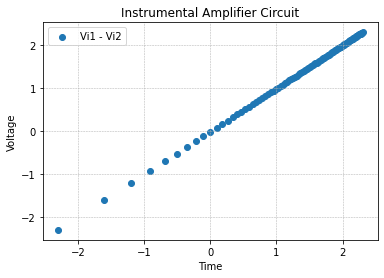
\includegraphics[scale = 0.8]{1.png}
\caption{$V_{out}$ vs ln($V_{in}$) after refining (ideal)}
\end{center}
\end{figure}




\section{Experimental results}
Our value of $V_{offfset}$, which came from the experimental IV data is -0.23V. But to make the $V_{out}$ vs ln($V_{in}$) graph to pass through (0,0), we have to malke the $V_{offfset}$ = -0.219V. \\
To make the slope of this graph as 1, we had to change the value of $R_2$ from 1k$\Omega $ (came by experimental analysis), to 1.1k$\Omega $. \\
So, because of changing $V_{offfset}$ from -0.23V to -0.219V, $a_2$ value changes from -0.46 to -0.438. \\
Due to changing of $R_2$ from 1k to 1.1k, $a_1$ value changes from -0.04862 to -0.05344. \\



\section{Experiment completion status}
All the parts of this experiment are completed successfully.

  

\end{document}
